\chapter{The history of sourdough}%
\label{ch:history}
\begin{quoting}
    We will start this book by briefly talking about the long history of
    sourdough bread from ancient time, and how people used similar process for
    other food like beer. The discovery of yeast and how, together with
    machine development, revolutionized bread making.  More recently
    communities formed around sourdough and home baking, trying to relearn
    lessons from the past.
\end{quoting}

The story of sourdough bread begins in prehistoric oceans. These oceans were the
birthplace of all life on Earth. To better envision the vast history of
our planet, lets create a timeline in one~year/365~days. On this scale,
January~1 signifies Earth's
formation 4.54~billion years ago. Midnight on December~31 is the present.
Each day represents roughly 12~million years. This technique simplifies the
complexity of time but also renders the extraordinary expanse of our planet's
history into a more graspable timeframe. We humans, are in fact a recent
addition to our planet, so young that we made our first appearance on
the evening of December~31.  It seems that humans managed to arrive just
in time to join the celebration at the end of the year.

On March~25, the oceans birthed the first single-celled bacteria. In these
waters, another single-celled life form, \emph{archaea}, also thrived. These
organisms inhabit extreme environments, from boiling vents to icy waters.

\begin{figure}[!htb]
\centering
  \begin{tikzpicture}
  % Draw horizontal line
  \draw[line width=1pt] (0,0) -- (\textwidth,0);

  % Define the width of each segment
  \pgfmathsetlengthmacro{\segmentwidth}{\textwidth/12}

  % Draw lines for the events, higher up so that they don't overflow the text
  % Placing the lines has been a bit manual work of trying different values
  % Maritime bacteria.

  \draw[line width=1pt] (2.8*\segmentwidth,1) -- (2.8*\segmentwidth,0.2);
  % Eukaryotes
  \draw[line width=1pt] (5.8*\segmentwidth,1.5) -- (5.8*\segmentwidth,0.2);
  % First bacteria on land
  \draw[line width=1pt] (9.1*\segmentwidth,-1.25) -- (9.1*\segmentwidth,-0.2);
  % Maritime fungi ancestors
  \draw[line width=1pt] (9.5*\segmentwidth,-2) -- (9.5*\segmentwidth,-0.2);
  % Fungi on land
  \draw[line width=1pt] (10.8*\segmentwidth,-2.75) -- (10.8*\segmentwidth,-0.2);
  % Yeasts on land
  \draw[line width=1pt] (11.1*\segmentwidth,-3.0) -- (11.1*\segmentwidth,-0.2);
  % First dinosaurs
  \draw[line width=1pt] (11.4*\segmentwidth,1) -- (11.4*\segmentwidth,0.2);
  % Dinosaur extinction
  \draw[line width=1pt] (11.9*\segmentwidth,1.5) -- (11.9*\segmentwidth,0.2);

  % Special lines for december events since they are so close togehter
  \draw[line width=1pt] (12.0*\segmentwidth,3.0) -- (12.0*\segmentwidth,0.2);  % Main branch
  \draw[line width=1pt] (12.0*\segmentwidth,3.0) -- (11.75*\segmentwidth,2.5); % Branch to first humans
  \draw[line width=1pt] (12.0*\segmentwidth,3.0) -- (11.75*\segmentwidth,3.0); % Branch to Jordan
  \draw[line width=1pt] (12.0*\segmentwidth,3.0) -- (11.75*\segmentwidth,3.5); % Branch to Pasteur

  % Draw months and month separators
  \foreach \i/\month in {0/Jan, 1/Feb, 2/Mar, 3/Apr, 4/May, 5/Jun, 6/Jul, 7/Aug, 8/Sep, 9/Oct, 10/Nov, 11/Dec} {
      % Separators
      \draw[line width=1pt] (\i*\segmentwidth,0.1) -- (\i*\segmentwidth,-0.1);
      % Month names
      \node[timeline_event, below] at ({(\i+0.5)*\segmentwidth},-0.1) {\month};
  }
  \draw[line width=1pt] (\textwidth,0.1) -- (\textwidth,-0.1);

  % Place events on the timeline with dates using the timeline_event style
  % As a calculation I used (4.54 billion years / 12 months = 0.3785 billion years/month.
  \node[timeline_event, above] at (2.0*\segmentwidth,1) {Mar 25 - First maritime bacteria and archae};
  \node[timeline_event, above] at (4.50*\segmentwidth,1.5) {June 25 - First organisms with nuklei (eukaryotes)};
  \node[timeline_event, above] at (7.8*\segmentwidth,-1.5) {Oct 4 - First bacteria on land};
  \node[timeline_event, above] at (8.0*\segmentwidth,-2.25) {Oct 15 - First maritime ancestors of fungi};
  \node[timeline_event, above] at (9.7*\segmentwidth,-2.75) {Nov 24 - Fungi on land};
  \node[timeline_event, above] at (10.5*\segmentwidth,-3.25) {Dec 3 - Yeasts on land};
  \node[timeline_event, above] at (10.25*\segmentwidth,1) {Dec 14 - First dinosaurs};
  \node[timeline_event, above] at (10.33*\segmentwidth,1.5) {Dec 29 - Dinosaurs go extinct};
  \node[timeline_event, above, anchor=east, align=right] at (11.75*\segmentwidth,2.5) {Dec 31 - First humans};
  \node[timeline_event, above, anchor=east, align=right] at (11.75*\segmentwidth,3.0) {Dec 31 - Sourdough in Jordan (23:59:55)};
  \node[timeline_event, above, anchor=east, align=right] at (11.75*\segmentwidth,3.5) {Dec 31 - Louis Pasteur isolated yeast (23:59:59)};

\end{tikzpicture}

  \caption[Sourdough microbiology timeline]{Timeline of significant events
    starting from the first day of Earth's existence,
    divided into months, and extending to the present day,
    marked at midnight. This visualization shows the pivotal steps
    of life and sourdough on earth.}%
  \label{fig:planet-timeline}
\end{figure}

Whoever comes first, bacteria or archaea, remains debated. For three
months (or approximately 1.1~billion years), these life forms dominated
the oceans. Then, on June~25 in an highly unlikely event, an archaeon consumed a bacterium.
Instead of digesting it, they formed a symbiotic relationship. This led to the
first nucleated organisms, marking an evolutionary milestone. This event lead
to the development of plants, fungi and also ultimately humans.

Life stayed aquatic for another three months.
On October~4, bacteria first colonized land. By October~15, the
first aquatic fungi appeared. They adapted and, by November~24, had colonized
land.

By December~3, yeasts emerged on land. This laid groundwork for bread-making.
Jump 140~million years to December~14, and dinosaurs arose. Just a couple
of days after their appearance on December~17 the super continent Pangea
started to rift apart, reshaping the continents into their current form.
The dinosaurs reigned until December~29 when they faced extinction.
Another 25~million years later, or our timeline's 2~days after the dinosaur
extinction, humans appeared.

A few hours later after the arrival of humans, a more subtle culinary
revolution was unfolding. By \num{12000}~BC, just 5 seconds before our metaphorical
midnight, the first sourdough breads were being baked in ancient Jordan. A blink of
an eye later, or 4~seconds in our time compression, Pasteur's groundbreaking work
with yeasts set the stage for modern bread-making. From the moment this book
began to take shape to your current reading, only milliseconds have ticked
by~\cite{Yong+2017}.

Now delving deeper into the realm of sourdough, it can likely be traced to aforementioned
Ancient Jordan~\cite{jordan+bread}. Looking at the earth's timeline sourdough
bread can be considered a very recent invention.

\begin{figure}[!htb]
\centering
  \begin{tikzpicture}
  % Draw horizontal line
  \draw[line width=1pt] (0,0) -- (\textwidth,0);

  % Define the width of each segment
  \pgfmathsetlengthmacro{\segmentwidth}{\textwidth/12}

  % Lines for periods
  \draw[stealth-stealth, line width=1pt] (0,-4.2)
    -- node[midway, timeline_timespan] {Historic breadmaking} ({\segmentwidth * 7.8},-4.2);
  \draw[stealth-stealth, line width=1pt] ({\segmentwidth * 7.8},-4.2)
    -- node[midway, timeline_timespan] {Modern bread} ({\segmentwidth * 12},-4.2);

  % Regularly placed events, not in chronological order
  % since should be placed on top of others on the timeline
  \draw[line width=1pt] ({\segmentwidth*3},1.5) -- ({\segmentwidth*3},0.3)
    node[at start, above, timeline_event] {6000 BC: First beer in Egypt};
  \draw[line width=1pt] ({\segmentwidth*5.95},2.5) -- ({\segmentwidth*5.95},0.3)
    node[at start, above, timeline_event] {70 BC:~First water mill};

  \draw[line width=1pt] ({\segmentwidth*10.50},2.5) -- ({\segmentwidth*10.50},0.3);
  \node[timeline_event, above, anchor=east] at ({\segmentwidth*12.50},2.5) {1950:~Modern Wheat};

  \draw[line width=1pt] ({\segmentwidth*11.20},-3.25) -- ({\segmentwidth*11.20},-0.3);
  \node[timeline_event, above, anchor=east] at ({\segmentwidth*12.20},-3.5) {2020~COVID-19 Pandemic};

    \draw[line width=1pt] ({\segmentwidth*9.60},1.5) -- ({\segmentwidth*9.60},0.3)
    node[at start, above, timeline_event] {1868:~Commercial yeast};
  \draw[line width=1pt] ({\segmentwidth*7.8},0.75) -- ({\segmentwidth*7.8},0.3)
    node[at start, above, timeline_event] {1680:~Discovery of microorganisms};
  \draw[line width=1pt] ({\segmentwidth*9.80},-2.5) -- ({\segmentwidth*9.80},-0.3)
    node[at start, below, timeline_event] {1885:~Electrical mixer};
  \draw[line width=1pt] ({\segmentwidth*9.57},-1.75) -- ({\segmentwidth*9.57},-0.3)
    node[at start, below, timeline_event] {1857:~Isolated Yeast};
  \draw[line width=1pt] ({\segmentwidth*8.80},-1.25) -- ({\segmentwidth*8.80},-0.3)
    node[at start, above, timeline_event] {1785:~Steam mill};

  % Lines to events
  % Cultivation of Einkorn
  \draw[line width=1pt] (0,1) -- (0,0.3);
  \draw[line width=1pt] (0,1) -- (0.25,1);
  \node[timeline_event, above, anchor=west] at (0.25,1) {12000 BC:~Cultivation of Einkorn};

  % Sourdough in Jordan
  \draw[line width=1pt] (0,-1) -- (0,-0.3);
  \draw[line width=1pt] (0,-1) -- (0.25,-1);
  \node[timeline_event, above, anchor=west] at (0.25,-1) {12000 BC:~Sourdough in Jordan};
  % Events

  % Indicators for period
  % Draw months and month separators
  \foreach \i/\month in {0/12000, 1/10000, 2/8000, 3/6000, 4/4000, 5/2000,
  6/0, 7/1600, 8/1700, 9/1800, 10/1900, 11/2000, 12/2100} {
      % Separators
      \draw[line width=1pt] (\i*\segmentwidth,0.1) -- (\i*\segmentwidth,-0.1);
      % Events for timeline
      \node[timeline_event, below] at ({(\i)*\segmentwidth},-0.1) {\month};
  }
\end{tikzpicture}

  \caption[Sourdough history timeline]{Timeline of significant discoveries and
  events leading to modern sourdough bread.}%
  \label{fig:sourdough-timeline}
\end{figure}

The exact origins of fermented
bread are, however, unknown. One of the most ancient preserved
sourdough breads has been excavated in Switzerland~\cite{switzerland+bread}.

\begin{figure}[ht]
  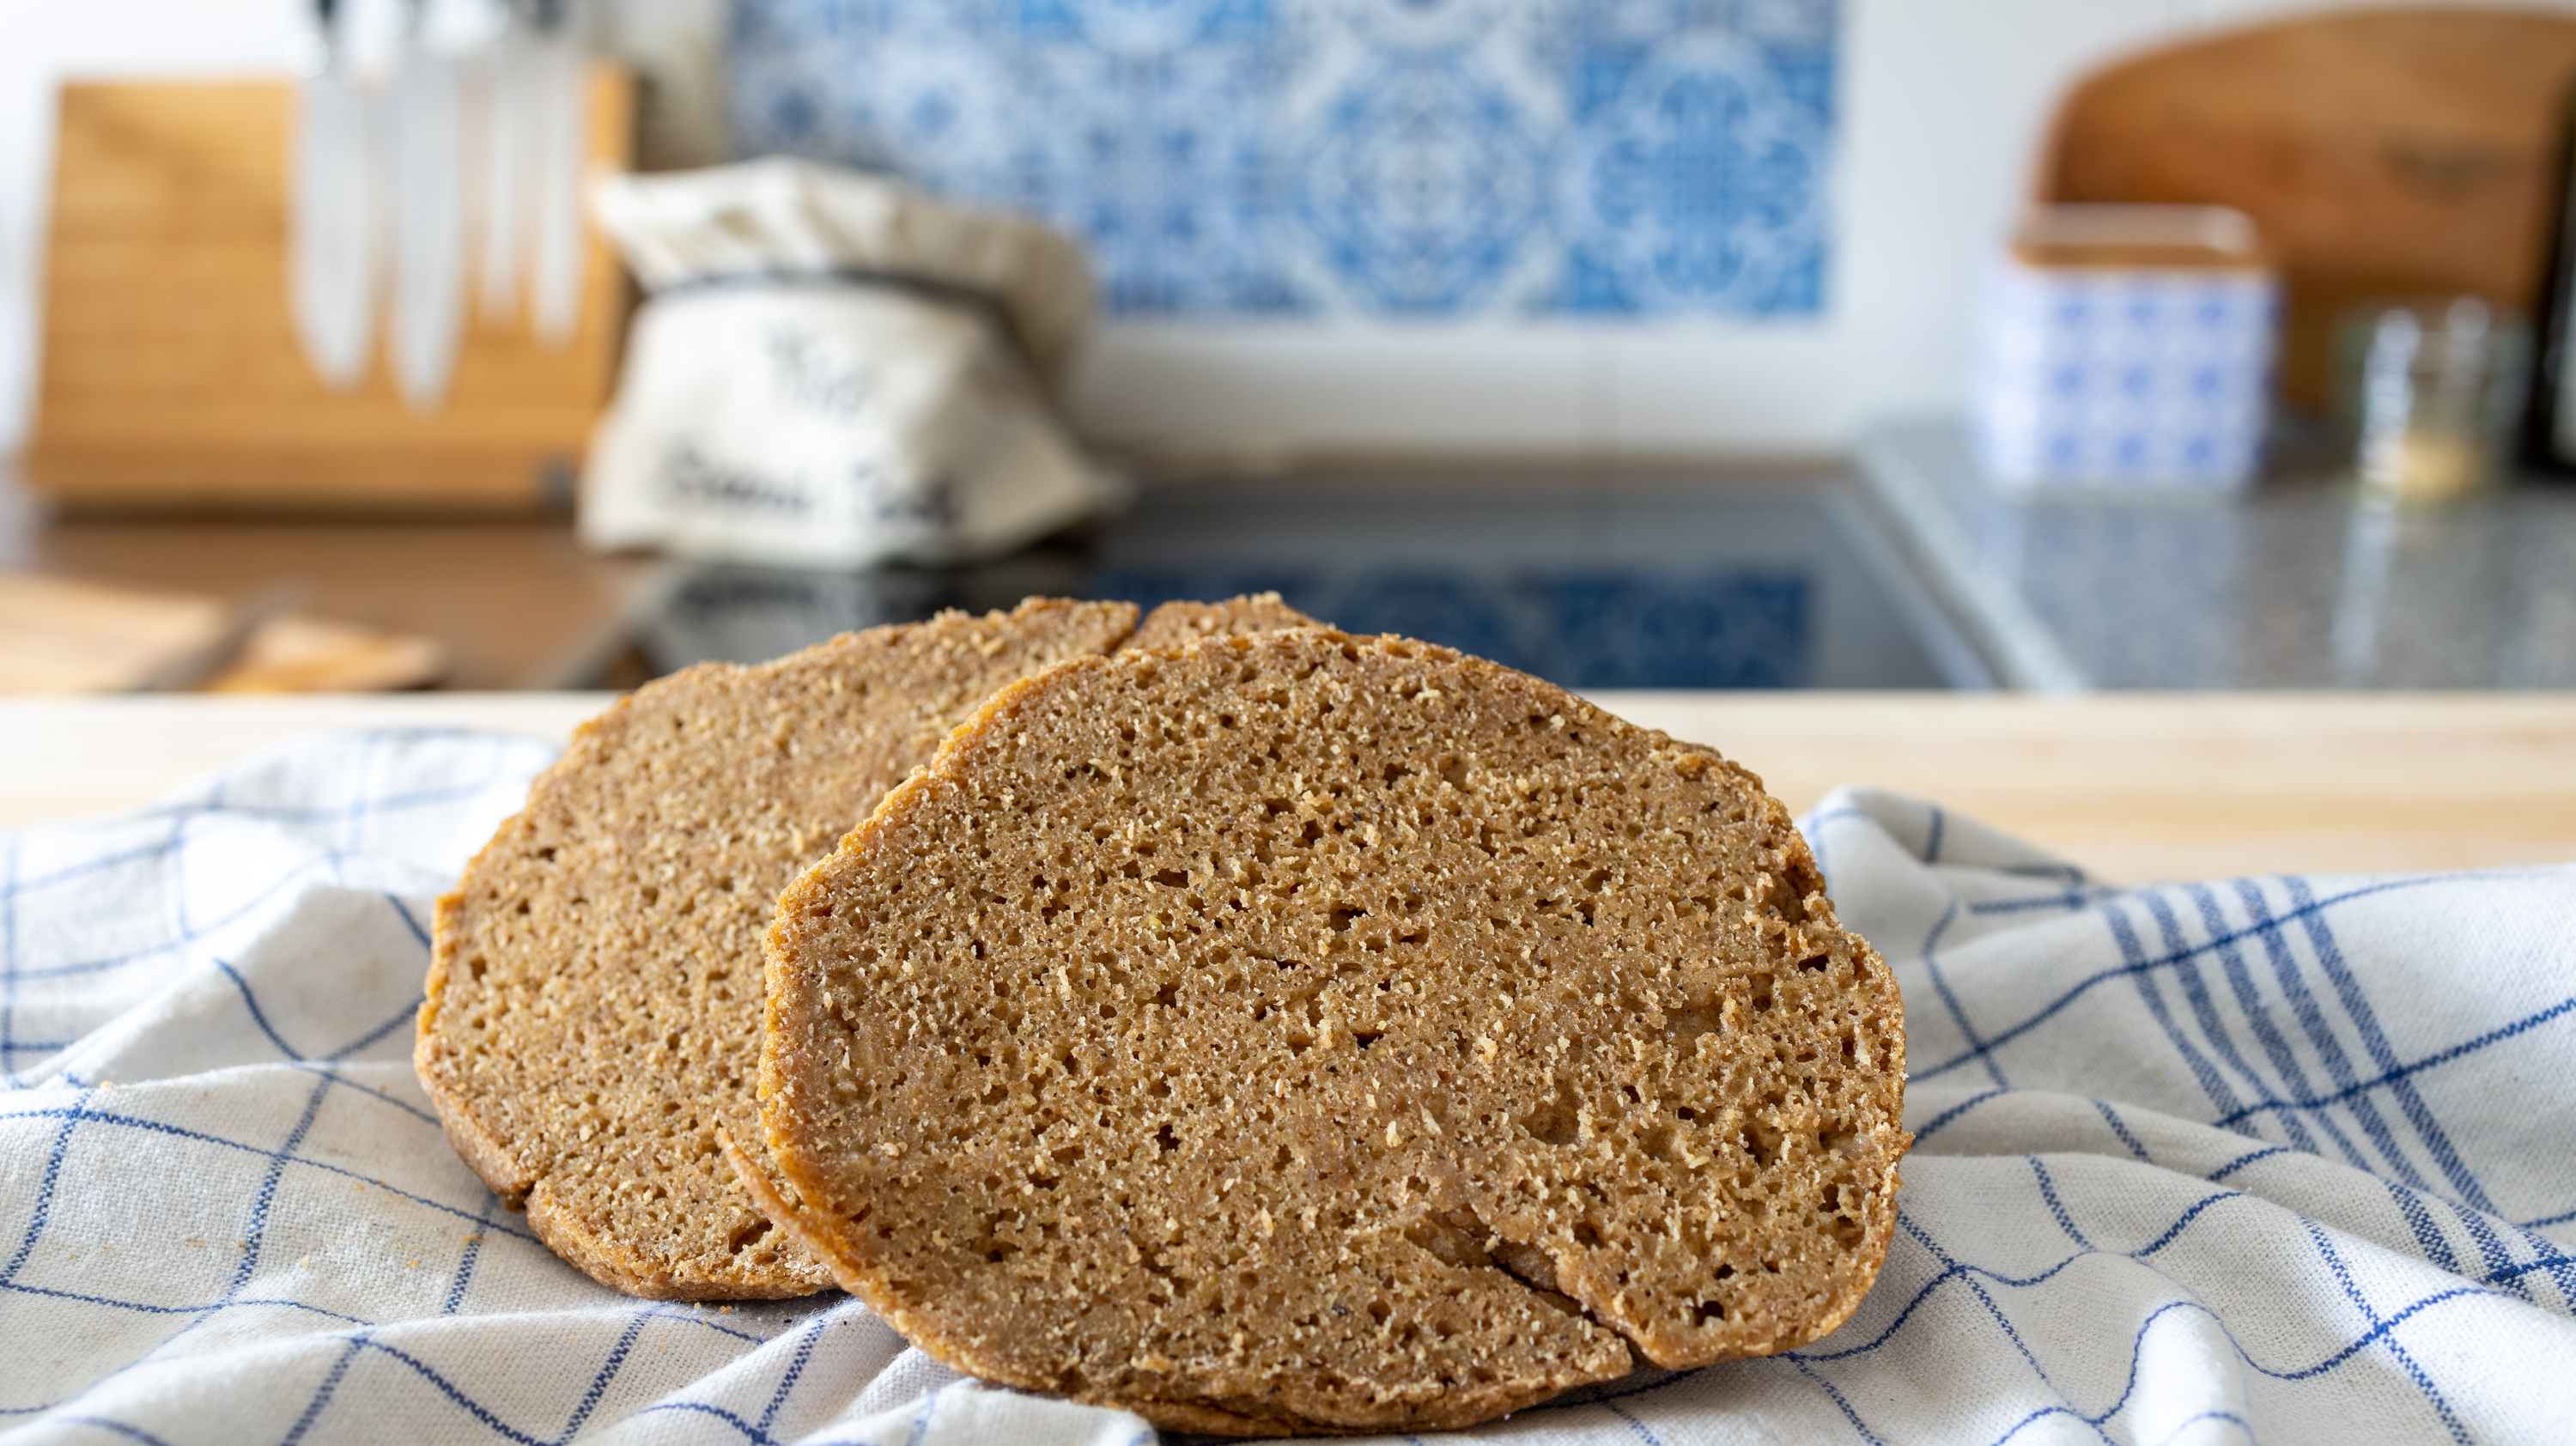
\includegraphics[width=\textwidth]{einkorn-crumb}
  \caption[Ancient Einkorn flatbread]{An ancient Einkorn flatbread. Note the
      dense crumb structure.}%
  \label{einkorn-crumb}
\end{figure}

Another popular story is that a lady in Egypt was making
a bread dough close to the Nile river. The lady forgot the
dough and at her return a few days later, she noticed that the dough had
increased in size and smelled funky. She decided to bake
the dough anyway and was rewarded with a much
lighter, softer, better tasting bread dough. From that day
on she continued to make bread this way~\cite{egyptian+bread}.

Little did the people back then know that tiny microorganisms
were the reason the bread was better. It is not clear when
they started using a bit of the dough from the previous
day for the next batch of dough. But by doing so, sourdough
bread making---as we know it today---was born: Wild yeast
in the flour and in the air, with bacteria
starting to decompose the flour-water mixture.
The yeast makes the dough fluffy,
and the bacteria primarily creates acidity. The different
microorganisms work in a symbiotic relationship. Humans
appreciated the enhanced airy structure and slight acidity
of the dough. Furthermore, the shelf life of such bread
was extended due to the increased acidity.

Quickly, similar processes were discovered when brewing beer
or making wine. A small tiny batch of the previous production
would be used for the next production. In this way, humans created
modern bread yeasts, wine yeasts, and beer yeasts~\cite{egypt+beer}.

Over time with each batch, the yeasts and bacteria
would become better at consuming whatever they were thrown at.
By feeding your sourdough starter, you are selectively breeding
microorganisms that are good at eating your flour. With
each iteration, your sourdough knows how to better ferment the flour
at hand. This is also the reason\footnote{It is crazy if you think about it.
People have been using this process despite not knowing what was going on for
thousands of years!} why more mature sourdough starters sometimes tend to
leaven doughs faster~\cite{review+of+sourdough+starters}.  The sourdough in
itself is a symbiotic relationship, but the sourdough
also adapted to humans and formed a symbiotic relationship with us.
For food and water, we are rewarded with delicious bread. In exchange,
we shelter and protect the sourdough. Spores from the starter
are spread through aerial contamination or insects like fruit flies.
This allows the sourdough starter to spread its spores even
further all around the world.

Evidence suggests early grain grinding in northern Australia around
\num{60000}~BC, notably at the Madjedbebe rock shelter in Arnhem
Land~\cite{aboriginal+grinding+stones}.  However, a more significant
advancement occurred later, as documented by the ancient Greek geographer
Strabo in \num{71}~BC\@.  Strabo's writings described the first water-powered
stone mill, known as a \emph{gristmill}. These mills advanced flour production
from a few kilograms up to several metric tons per day~\cite{history+mills}.

These early mills featured horizontal paddle wheels, eventually termed
\emph{Norse wheels} due to their prevalence in Scandinavia.  The paddle wheels
connected to a shaft, which, in turn, linked to the central runner stone for
grinding. Water flow propelled the paddle wheels, transferring the grinding
force to the stationary \emph{bed}, typically a stone of similar size and
shape. This design was straightforward, avoiding the need for gears. However,
it had a limitation: the stone's rotation speed relied on water volume and
flow rate, making it most suitable for regions with fast-flowing streams,
often found in mountainous areas~\cite{mills+scandinavia}.

In the year \num{1680}, a remarkable scientist by the name of
Antonie~van~Leeuwenhoek introduced a groundbreaking innovation that would
forever alter our understanding of the microscopic world and ultimately bread
making.  Van~Leeuwenhoek, a master of lens craftsmanship, possessed an
insatiable fascination with realms invisible to the naked eye. His pioneering
work birthed the first modern microscope.  What set Van~Leeuwenhoek apart was
the exceptional quality of his lenses, capable of magnifying tiny
microorganisms by an astounding factor of \num{270}.  Driven by an unrelenting
curiosity to unveil the unseen, he embarked on a journey of exploration. He
scrutinized flies, examined lice-infested hair, and ultimately turned his gaze
toward the tranquil waters of a small lake near Delft.

In this serene aquatic habitat, he made astonishing observations, discovering
algae and minuscule, dancing creatures hitherto hidden from human perception.
Eager to share his revelatory findings with the scientific community,
Van~Leeuwenhoek faced skepticism, as it was difficult to fathom that someone
had witnessed thousands of diminutive, dancing entities—entities so tiny that
they eluded the human eye.

Undeterred by skepticism, he continued his relentless pursuit of the unseen,
directing his lens towards a brewer's beer sludge. In this obscure medium,
Van~Leeuwenhoek made history by becoming the first human to lay eyes upon
bacteria and yeast, unraveling a previously concealed world that would
revolutionize our understanding of microbiology~\cite{Yong+2017+Leeuwen}.

At the same time brewers would start to experiment with utilizing the muddy
leftovers of the beer fermentation to start making doughs. They would notice
that the resulting bread doughs were becoming fluffy and compared
to the sourdough process would lack the acidity in the final product.
A popular example is shown in a report from \num{1875}. Eben Norton Horsford
wrote about the famous \emph{Kaiser Semmeln} (Emperor's bread rolls).
These are essentially bread rolls made with brewer's yeast instead
of the sourdough leavening agent. As the process is more expensive,
bread rolls like these were ultimately consumed by the noble people
in Vienna~\cite{vienna+breadrolls}.

As industrialisation began the first steam-powered grain mill was developed by
Oliver Evans in \num{1785}. Evans' design incorporated several innovations,
including automated machinery for various milling processes, making it more
efficient than traditional water or animal-powered mills. His steam-powered
mill marked a significant advancement in industrial technology for bread
making~\cite{evans+mill}.

\begin{figure}[ht]
  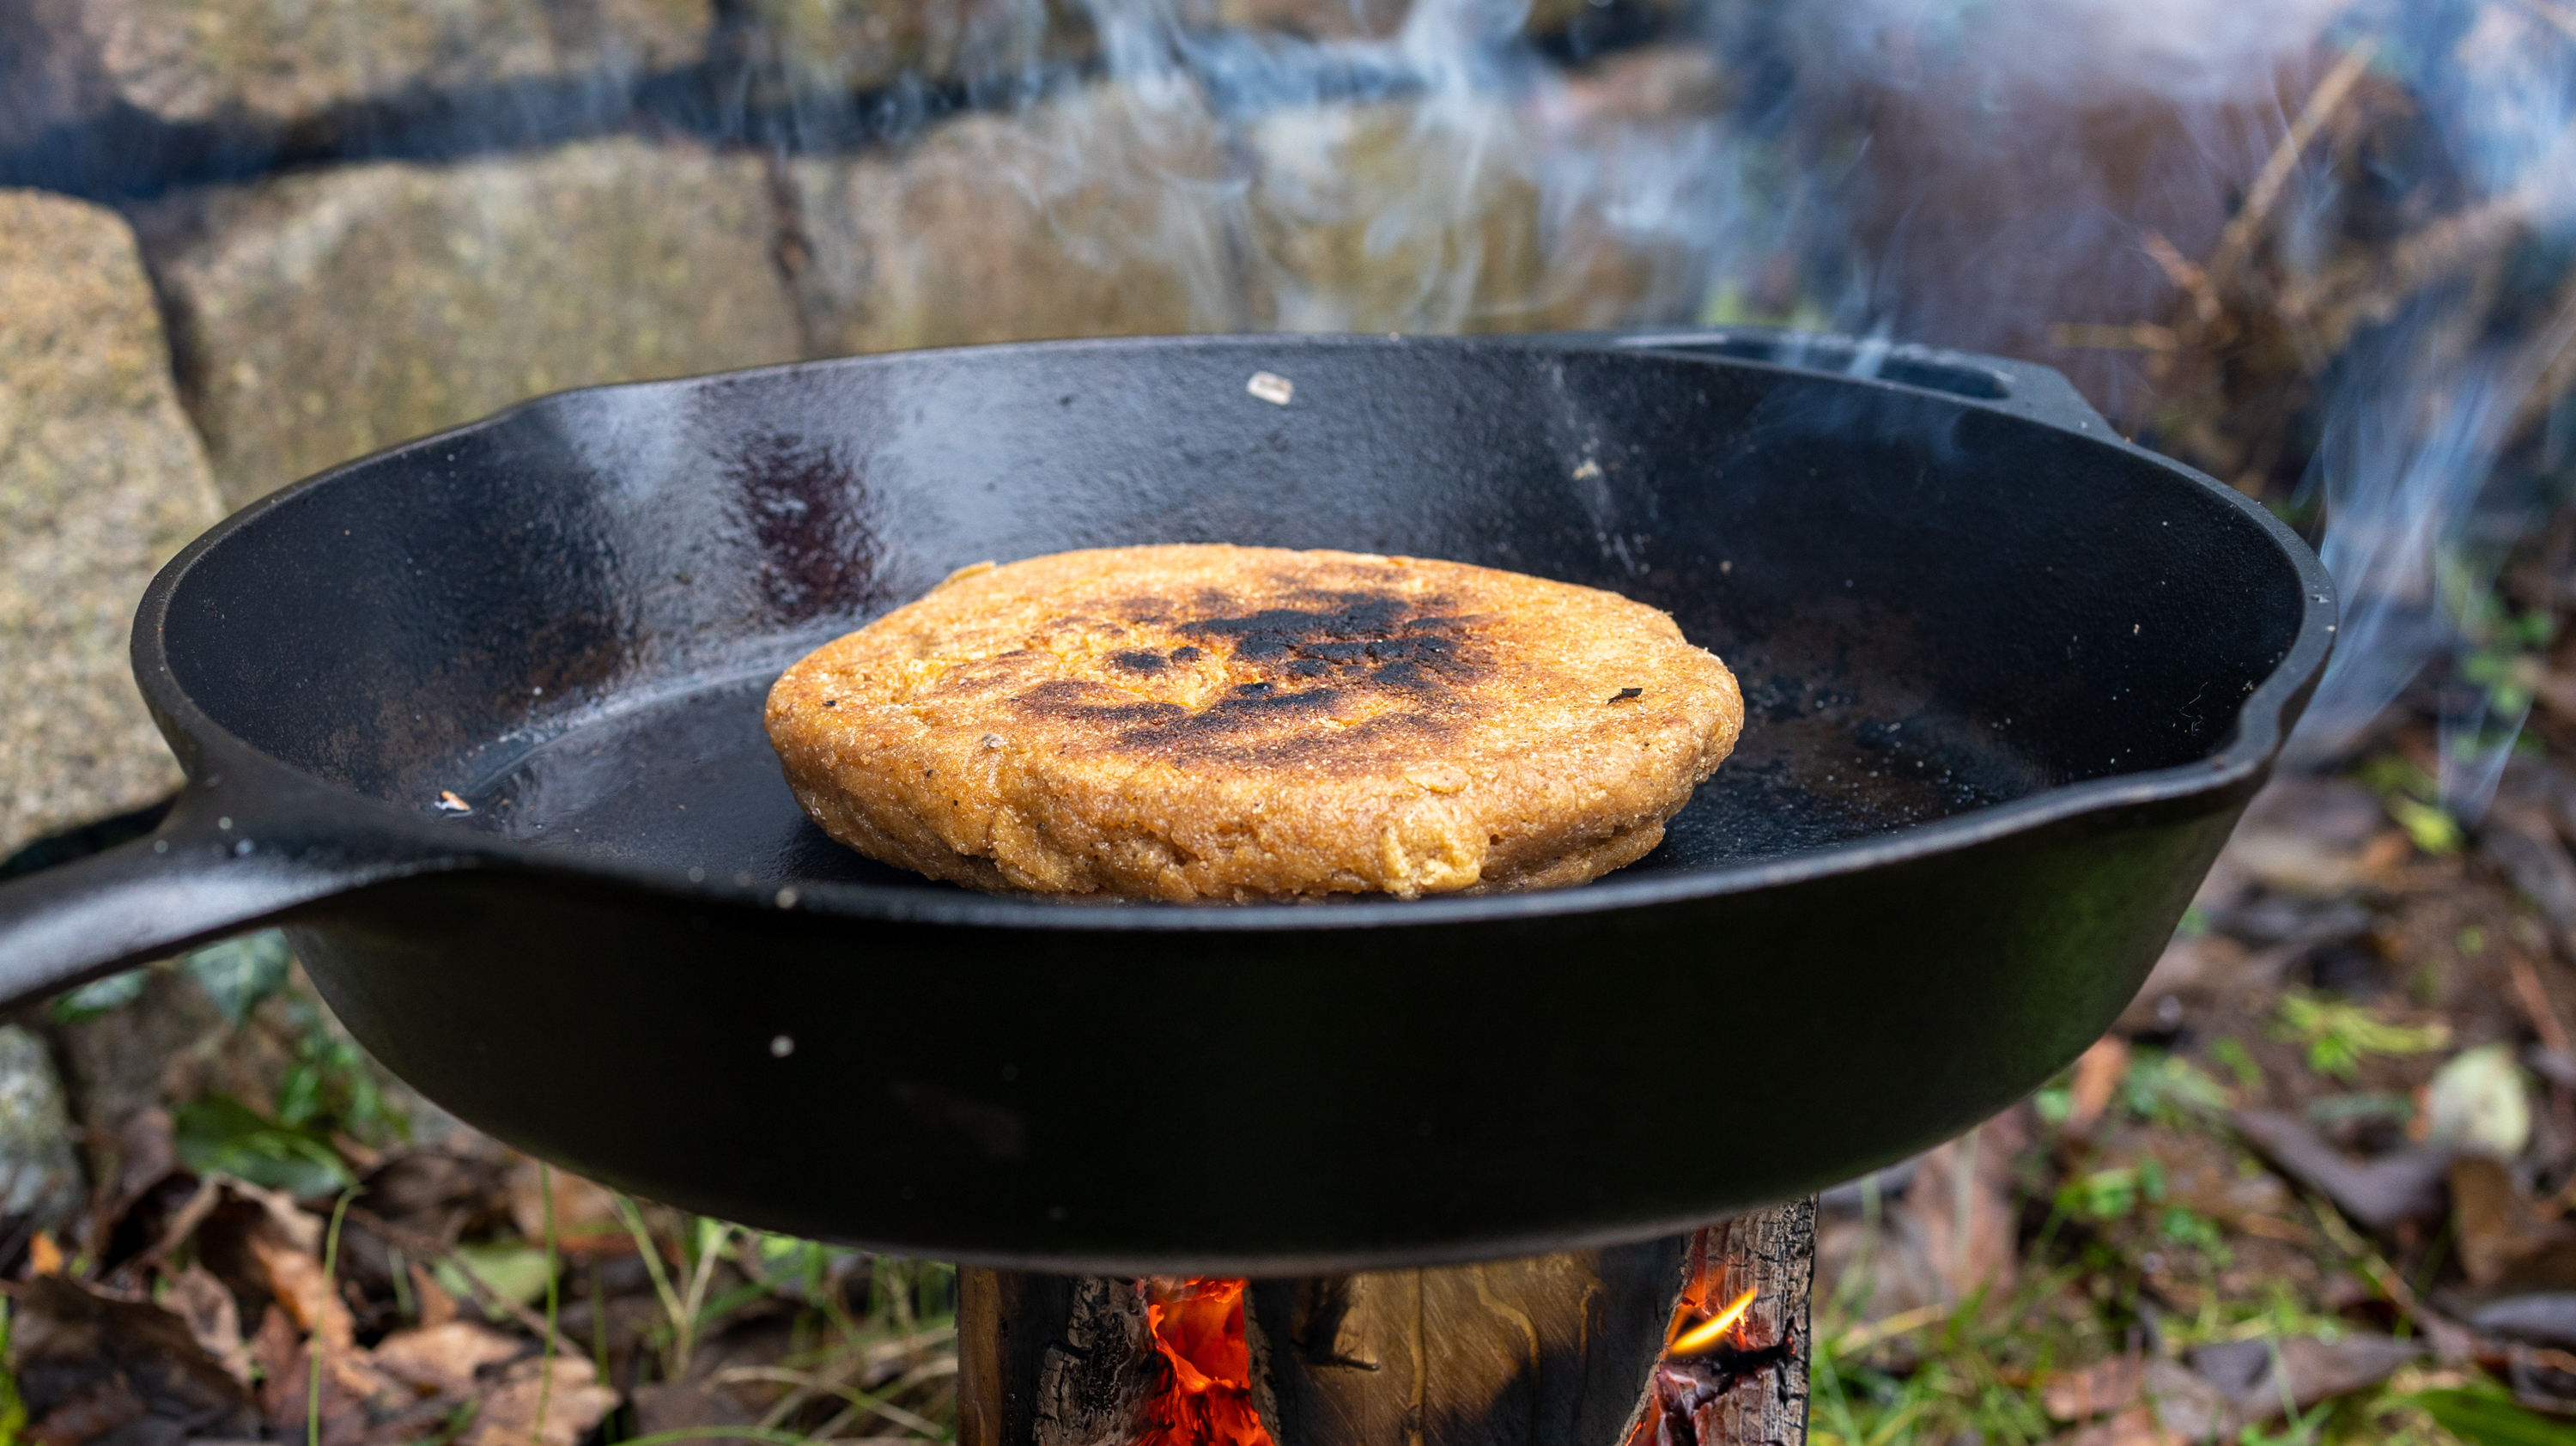
\includegraphics[width=\textwidth]{sourdough-stove}
  \caption{A bread made over the stove without an oven.}%
  \label{sourdough-stove}
\end{figure}

The biggest advancement of industrial breadmaking happened in \num{1857}.
The French microbiologist Louis Pasteur discovered
the process of alcoholic fermentation. He would prove that
yeast microorganisms are the reason for alcoholic fermentation
and not other chemical catalysts. He continued with his research and
was the first person to isolate and grow pure yeast strains.
Soon later in \num{1868} in the Fleischmann brothers Charles
and Maximilian were the first to patent pure yeast strains
for bread making. The yeasts offered
were isolated from batches of sourdough. By \num{1879} the machinery was built
to multiply the yeast in large centrifuges~\cite{fleischmann+history}.
The pure yeast would prove to be excellent and turbocharged
at leavening bread doughs. What would previously take 10~hours
to leaven a bread dough could now be done within 1~hour.
The process became much more efficient. What ultimately made making large
batches of dough possible, was the invention of the electrical kneader.  Rufus
Eastman, an American inventor, is often credited with an important advancement
in mixer technology. In \num{1885}, he received a patent for an electric mixer
with a mechanical hand-crank mechanism.  This device was not as advanced or as
widely adopted as later electric mixers, but it was an early attempt to
mechanize mixing and kneading processes in the kitchen using electricity.
Eastman's invention represented an important step in the development of
electric mixers, but it wasn't as sophisticated or popular as later models
like the KitchenAid mixer. The KitchenAid mixer, introduced in \num{1919}, is
often recognized as one of the first widely successful electric mixers and
played a significant role in revolutionizing kitchen appliances for home
cooks~\cite{first+mixer}~\cite{kitchenaid+history}.

During World~War~II the first packaged dry yeast was developed. This would
ultimately allow bakeries and home bakers to make bread much faster and more
consistently. Thanks to pure yeast, building industrial bread making machines
was now possible. Provided you maintain the same temperature, same flour and
yeast strains fermentation became precisely reproducible. This ultimately lead
to the development of giga bakeries and flour blenders. The bakeries demanded
the same flour from year to year to bake bread in their machines.  For this
reason, none of the supermarket flour you buy today is single origin.  It is
always blended to achieve exactly the same product throughout the years.

Modern wheat, specifically the high-yielding and disease-resistant varieties
commonly grown today, began to be developed in the mid-20th century. This
period is often referred to as the \emph{Green Revolution.}

One of the key figures in this development was American scientist Norman
Borlaug, who is credited with breeding high-yield wheat varieties,
particularly dwarf wheat varieties, that were resistant to diseases and could
thrive in various environmental conditions. His work, which started in the
1940s and continued through the \num{1960}s, played a crucial role in
increasing wheat production worldwide and alleviating food
shortages~\cite{green+revolution}.

As fermentation
times sped up, the taste of the final bread would deteriorate.
The sprouting process induced by certain enzymes is essential
to developing a fluffier texture and better tasting crust. This
can't be indefinitely sped up. Soon bakeries would start
to introduce additional enzymes to achieve similar properties
to sourdough bread in yeast-based doughs. Sourdough almost completely
vanished from the surface of the Earth. Only a handful
of true nerds would continue making bread with sourdough.

Suddenly people started to talk more often about celiac disease
and the role of gluten. The disease isn't new; it has first
been described in \num{250}~AD~\cite{coeliac+disease}. People
would note how modern bread has much more gluten compared
to ancient bread. The bread in ancient times probably was much flatter.
The grains over time have been bred more and more towards containing a higher
amount of gluten. Gluten is a protein that gives modern
bread its typical soft fluffy crumb structure. The
gluten proteins bind together once activated with water.
Throughout the course of the fermentation, \ch{CO2} is trapped
in this protein matrix. The tiny created chambers expand
during the baking process. As the dough gelatinizes while
being heated, the structure is fortified. This makes the bread appear
soft and fluffy when tasting it. Similar to drinking raw cow's milk,
your immune system might react to the consumed proteins.
There is gluten intolerance
and celiac disease. When people say they don't handle
gluten well, it's mostly a gluten intolerance they describe.
Some people describe similar issues when consuming
too much lactose. If you eat a long-fermented cheese
however, most of the lactose has been fermented by
the tiny microorganisms. People would investigate and
note how sourdough bread can typically be handled better
compared to plain, fast-made factory bread. The
reason for this is that enzymes take time to work the dough.
Gluten is a storage protein of flour. Once
sprouting is activated by adding water, the protease
enzyme starts to convert the gluten into tinier amino acids
that are required for sprouting. Over time you are effectively
losing gluten as it's naturally broken down. Furthermore,
traditionally lactic acid bacteria would start to decompose
the flour-water mix. Almost everything is recycled in nature.
Part of their diet is to consume the proteins in the dough.
Modern bread is faster and no longer has lactic acid bacteria.
Both factors together mean that you are consuming products
with a much higher gluten value compared to ancient times
when natural fermentation was used~\cite{raffaella+di+cagno}.

During the California Gold Rush, French bakers brought the sourdough
culture to Northern America. A popular bread became the
San Francisco sourdough. It's characterized by its unique
tang (which was previously common for every bread). It
however remained more of a niche food while industrial bread
was on the rise. What really expedited
the comeback of sourdough was the \num{2020} COVID-19 pandemic.
Flour and yeast became scarce in the supermarkets. While
flour returned yeast couldn't be found. People started
to look for alternatives and rediscovered the ancient
way of making sourdough bread. Soon many realized
that making sourdough bread is more complex than modern
yeast-based bread. You need to maintain a sourdough starter
and have it in ideal shape to properly ferment your dough.
Furthermore, compared to a yeast-based dough, you can't just
punch the dough down and let the fermentation continue.
You can overferment your dough, resulting in a sticky
dough mess. This complexity led to many bakers looking
for help and many thriving communities formed around
the topic of homemade bread.

When interviewing Karl de~Smedt (owner of the Sourdough
Library) he said something that changed my way of thinking
about bread: ``The future of
modern bread is in the past~\cite{interview+karl+de+smedt}.''
